\documentclass{article}
\usepackage[spanish]{babel}
\usepackage[utf8]{inputenc}
\usepackage[nonatbib]{../template}

\usepackage[utf8]{inputenc} % allow utf-8 input
\usepackage[T1]{fontenc}    % use 8-bit T1 fonts
\usepackage{hyperref}       % hyperlinks
\usepackage{url}            % simple URL typesetting
\usepackage{booktabs}       % professional-quality tables
\usepackage{amsfonts}       % blackboard math symbols
\usepackage{nicefrac}       % compact symbols for 1/2, etc.
\usepackage{microtype}      % microtypography
\usepackage{xcolor}         % colors
\usepackage{graphicx}
\usepackage{float}
\usepackage[backend=biber,sorting=ynt,style=apa]{biblatex}

\addbibresource{../bibliography.bib}

\graphicspath{ {../imagenes/} }

\title{Entrega 2: Metodología y EDA}

\author{%
  José Saint Germain\\
  \texttt{josesg998@gmail.com} \\
}

\begin{document}

\maketitle

\section{Introducción}
El objetivo de esta entrega es realizar una breve descripción de las metodologías 
que se utilizarán durante el trabajo final de especialización, así como realizar 
un análisis exploratorio de los datos (EDA), para comprender mejor la estructura 
de los datos que se trabajarán.

\section{Metodología}
Como lo que buscamos realizar es experimentar con diferentes datos el mismo 
trabajo realizado por el FMI (\cite{Ceb24}), vamos a replicar las mismas 
técnicas de optimización de hiperparámetros, así como los mismos algoritmos
de entrenamiento y de intepretación de resultados.
 
% TODO incluyo explicación de los algoritmos?
Los algoritmos que se utilizarán serán Random Forest (\cite{Bre01}) y XGBoost
(\cite{Che16}). Adicionalmente, para la evaluación de performance se utilizará 
el área bajo la curva (AUC), en donde un valor de AUC de 0.5 indica que el modelo 
no tiene capacidad predictiva, mientras que un valor cercano a 1 indica que el 
modelo es capaz de predecir con alta precisión. Con respecto al ajuste de 
hiperparámetros se utilizará la optimización bayesiana. La misma consistirá en 100 
iteraciones en donde se buscará el valor óptimo de los siguientes hiperparámetros:

% agregar lista de viñetas
\begin{itemize}
  \item Random Forest: profundidad máxima de los árboles (max\_depth) y la 
  submuestra del ratio de columnas a considerar cuando se construye cada árbol 
  (max\_features).
  \item XGBoost: la tasa de aprendizaje (learning\_rate) y el término de 
  regularización L2 en los pesos (reg\_lambda).
\end{itemize}

Adicionalmente el parámetro que establece la cantidad de árboles creados 
(n\_estimators) quedará fijado en 1000.

Para evitar el data leakage, en cada iteraciónd de la optimización bayesiana
se utilizará la validacón cruzada. Sin embargo, como se trabajará con una base
de datos de panel, conviene utilizar una versión adaptada: el método \textit{block-
time-series cross-validation}, basado en \cite{Bur94} y \cite{RAc00}. El método 
aplicado en este caso consiste en generar 5 pares de entrenamiento y validación: 
{1970 - 2009, 2010 - 2011}; {1970 - 2011, 2012 - 2013}; {1970 - 2013, 2014 - 2015}; 
{1970 - 2015, 2016 - 2017}; {1970 - 2017, 2018- 2019}. Por lo tanto, cada set de 
entrenamiento consiste en observaciones desde 1970 hasta un añ de corte (2009, 
2011, 2013, 2015, 2017) y el set de validación contempla los dos años siguientes 
del mismo.

% TODO incluir explicacíón de los Shapley Values
Una vez realizada la optimización bayesiana, se toman los valores de hiperparámetros
que lograron maximizar el AUC y se entrena el modelo con el set de entrenamiento 
para intentar predecir los golpes de estado entre 2020 y 2022. Por último, para 
intepretar las variables más importantes en la predicción de golpes de estado, se 
utilizarán los valores Shapley (\cite{Str10}; \cite{Lun17}). Basado en la teoría de 
juegos, los valores Shapley buscan medir la contribución de cada predictor aa la 
probabilidad de un golpe en relación con la probabilidad promedio de la muestra 
prevista de un golpe.

\section{Análisis Exploratorio de Datos}

Como primera aproximación a la base de datos de Varieties of Democracy o V-Dem 
(\cite{CopMet24}), pasaremos a explicar la manera en que se construye la misma. Las
variables centrales se obtienen a partir de encuestas suministradas a expertos
sobre los distintos países. Inicialmente, se busca que cada país cuente con al menos
cinco expertos. Actualmente, la institución cuenta con 22 expertos promedio por país
y 7,1 experots por combinación de variable y país. Una vez obtenida las respuestas
de los expertos, se pasa al proceso de agregación para así conformar una base de 
datos donde cada fila corresopnda a un país en un año específico. De esta agregación
obtienen diferentes versiones de la misma variable:

\begin{itemize}
  \item Estimador del modelo (Variable sin sufijo): es la medida
   recomendada para su análisis. Corresponde a obtener la mediana del valor de 
   la variable entre los expertos, reescalado a valores entre -5 a 5.
  \item Medidas de incertidumbre (*\_codelow y *\_codehigh): corresponden a un 
  desvío estandar por encima y por debajo del estimador del modelo. 
  Usadas conjuntamente, construyen un intervalo de confianza del 95\%.
  \item Escala original (*\_osp): mediana de la variable, pero sin reescalar. Esta
  versión también cuenta con sus medidas de incertidumbre correspondientes.
  \item Media simple (\_mean): mediana de la variable, pero sin reescalar.
  \item Desvío estándar (\_sd): desvío estándar de la variable.
  \item Media simple (\_mean): media de la variable.
  \item Cantidades de expertos (\_nr): cantidad de expertos que respondieron por
  país, año y variable.
\end{itemize}

Podemos mencionar que la base cuenta con 27734 filas y 4607 columnas. Como es una 
base de datos de panel, se tiene información de 202 países durante 235 años. Las 
variables cuentan con un tipo de codificación particular que permite identificar el 
origen de la  variable. En primer lugar, el primer prefijo es indicativo de si fue 
producido por V-Dem o no:

\begin{itemize}
  \item v2: variables de V-Dem.
  \item v3: variables pertenecientes a la base V-Dem histórica.
  \item v2x\_: Índices principales e índices componentes.
  \item v2x\brackettext{indicador de dos letras}: Índices específicos de ciertas 
  áreas (ver más abajo).
  \item e\_: variables no generadas por V-Dem y variables V-Dem en versión ordinal.
\end{itemize}

El nombre de la variable también permite identificar la área temática a la que 
pertenece:

\begin{itemize}
  \item ca: Espacio cívico y académico
  \item cl: Libertad civil
  \item cs: Sociedad civil
  \item dd: Democracia directa
  \item de: Demografía
  \item dl: Deliberación
  \item el: Elecciones
  \item ex: Ejecutivo
  \item exl: Legitimación
  \item ju: Poder judicial
  \item leg: Legislatura
  \item lg: Legislatura
  \item me: Medios de comunicación
  \item pe: Igualdad política
  \item ps: Partidos políticos
  \item sv: Soberanía
  \item st: Estado
  \item x: Índice (calculado a partir de variables que también se 
  incluyen en la base de datos)
  \item zz: Cuestionario posterior a la encuesta
  \item ws: Encuesta de sociedad digital
\end{itemize}

A la base original obtenida desde la librería de V-Dem, se le realizaron los
siguientes filtros: en primer lugar, se removieron todas las variables que
no sean las principales, es decir, que no cuenten con sufijo. De esa manera,
se busca reducir el tamaño de la base y así poder agregar nuevas columnas
mediante ingeniería de atributos. En segundo lugar, se filtraron los años 
superiores a 1950, para adecuarnos al periodo utilizado en el artiçulo del FMI.
De esa manera, la base filtrada cuenta con 12208 filas y 1460 columnas. Por último,
se remueven todas las variables de fuentes externas (cuyo agrupador comienza con
'e'), las variables pertenecientes a la base histórica (agrupador 'hist') y las
de la encuesta de sistema de partidos políticos; en parte debido a que provienen
de fuentes agenas a V-Dem que pueden comprometer la completitud futura de los datos
y en parte porque algunas de estas variables cuentas con alta tasa de nulos.

\subsection{Ánalisis de nulos}

\begin{figure}[H]
  \centering  
  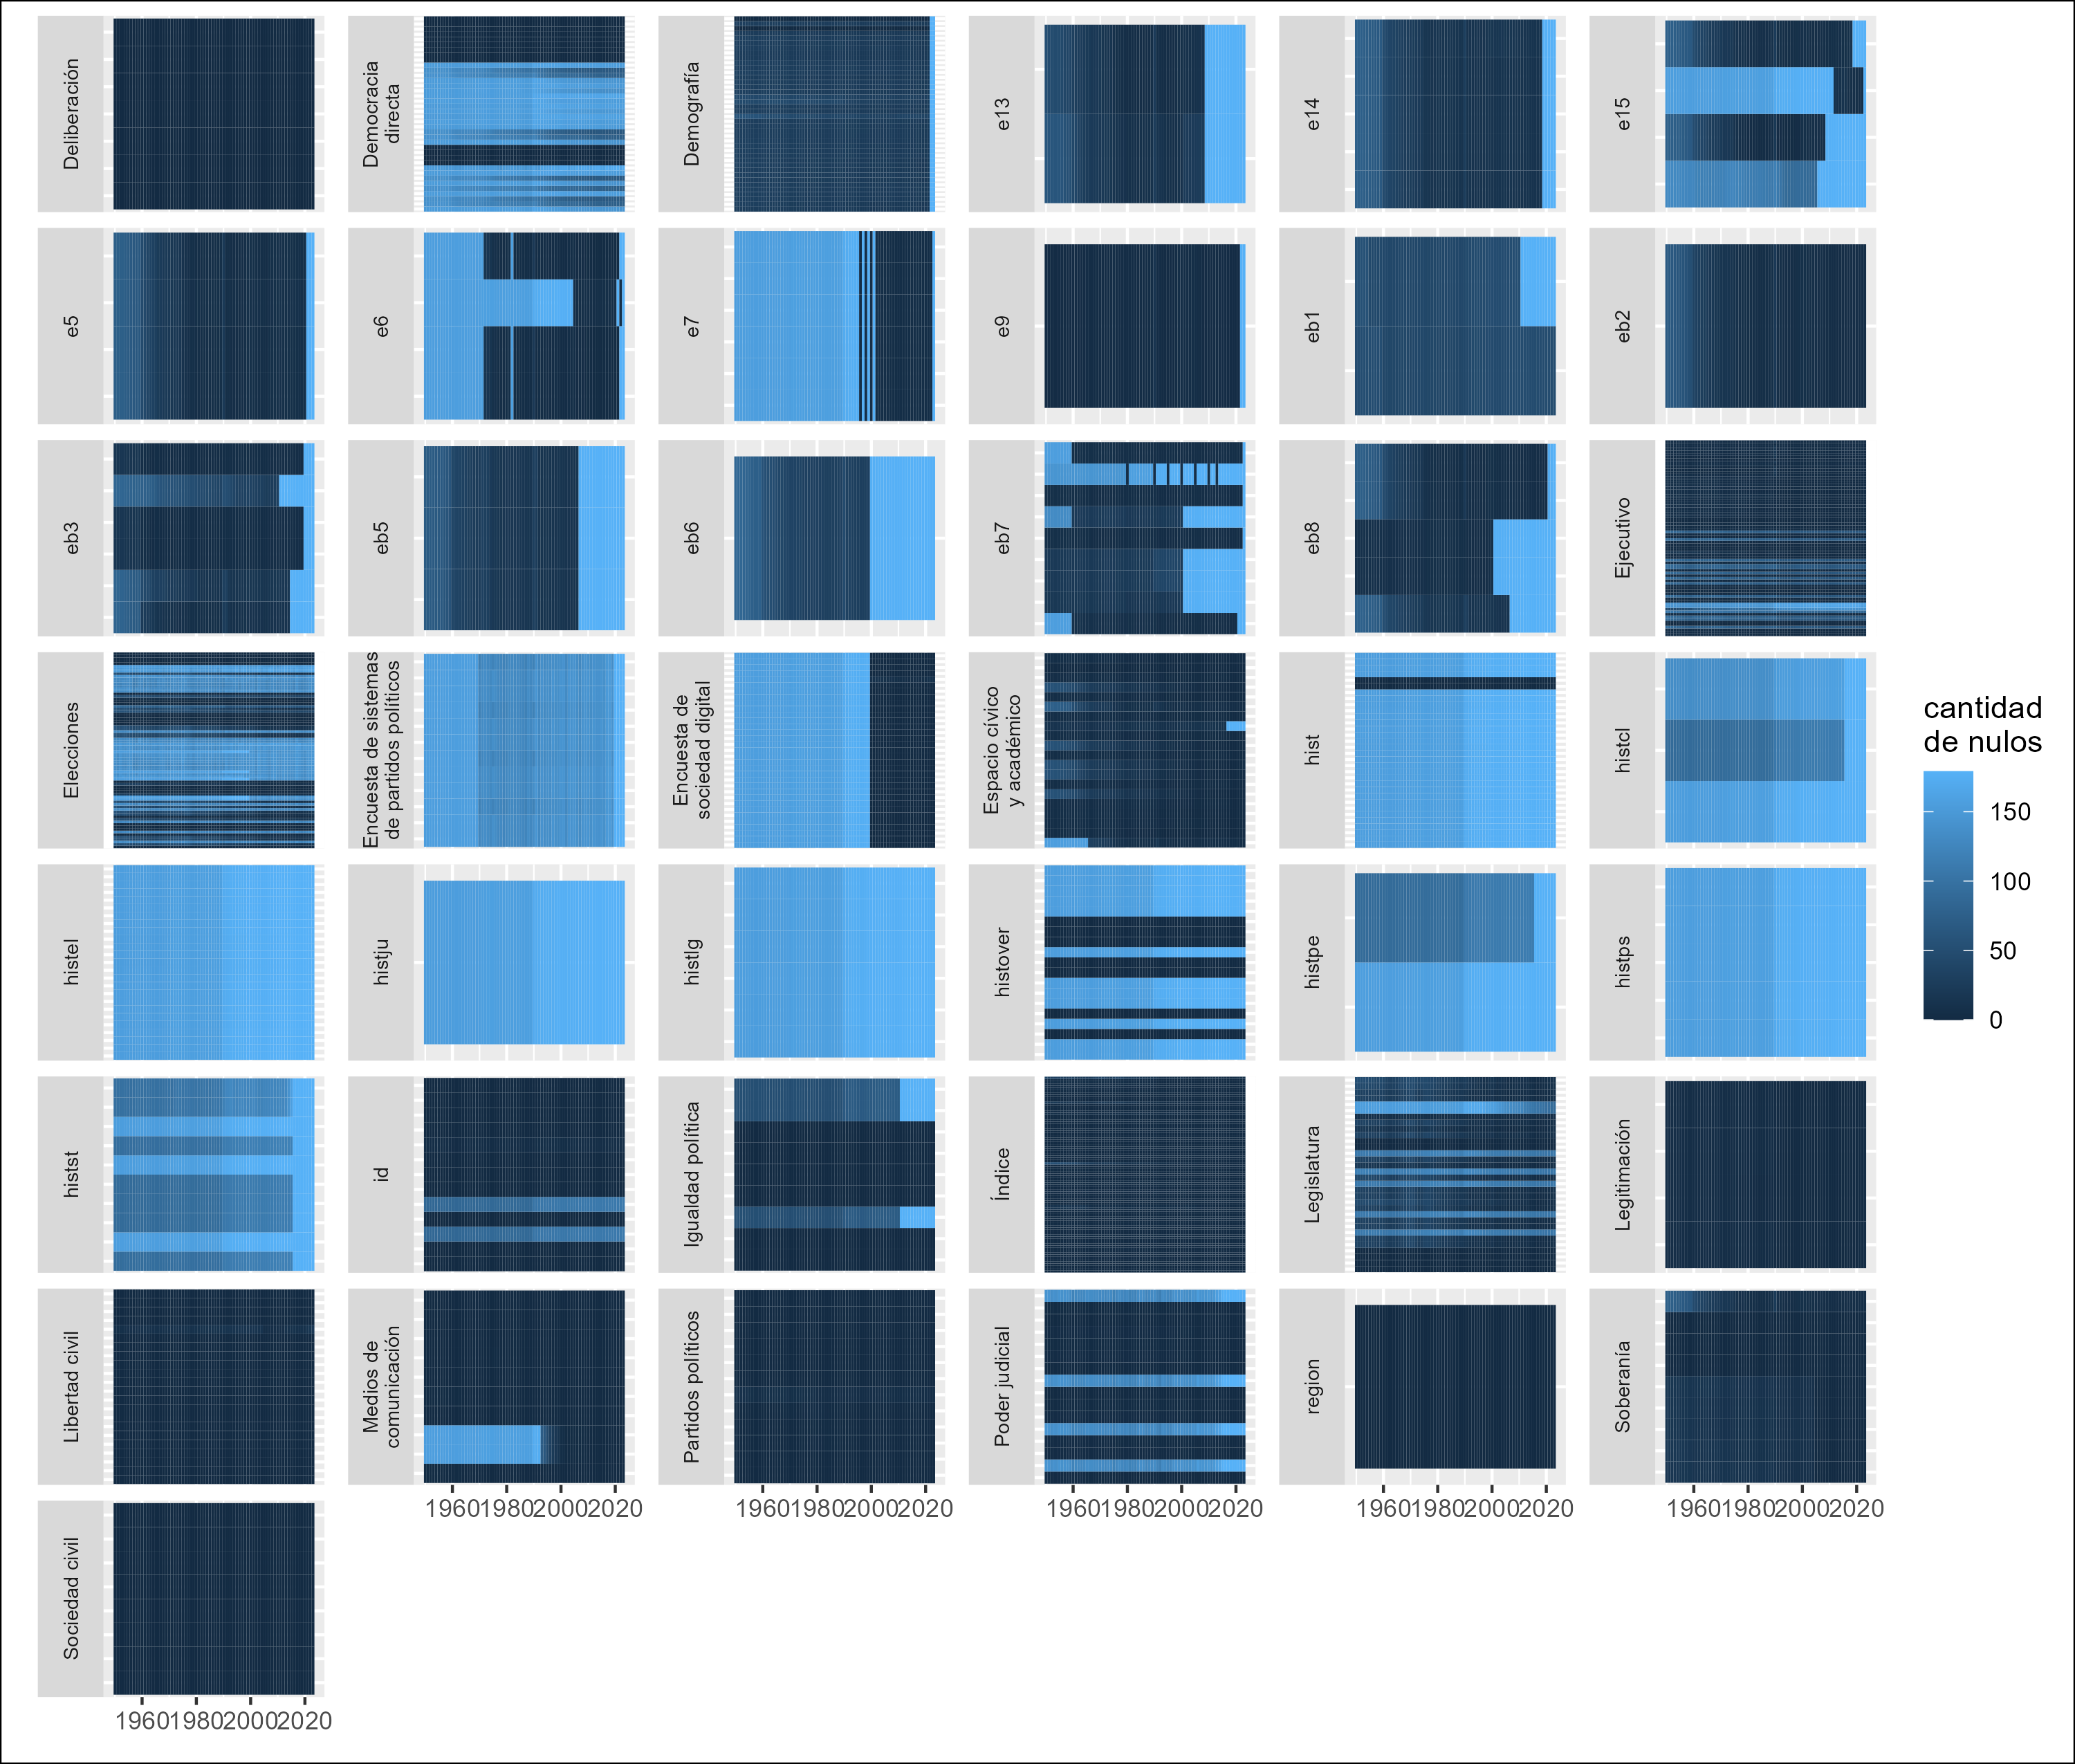
\includegraphics[width=1\textwidth]{1_nas.png}
  \caption{Conteo de nulos por año y agrupador de variables\label{fig:nas}}
\end{figure}

Debido a la alta cantidad de variables, no es posible realizar un análisis
pormenorizado de la presencia de nulos en cada una. Por ese motivo, se decidió
visualizar la misma mediante los agrupadores de variables con las que cuenta el
codebook de V-Dem. El mismo, discrimina las variables a partir de sus temas en 
común. De esa manera, en la figura ~\ref{fig:nas} la cantidad de nulos por 
categoría de variable expresado en un mapa de calor, donde cada fila es una 
variable individual y las columnas los diferentes años del panel.

De este gráfico podemos aprehender ciertos patrones sobre la presencia de nulos
en algunos grupos de variables: En primer lugar, observamos variables que,
anteriormente a un año puntual, no cuentan con información. En este ejemplo caen
las variables sobre governanza otorgadas por el banco mundial (e7), las preguntas
pertenecientes a la encuesta de sociedad digital (wsmcio), variables referentes a
la libertad en medios digitales (wsmdmf), las referntes a la polarización en medios
online (wsmomp) y las referentes a clivajes sociales (wsmsc).

En segundo lugar, figuran casos contrarios, en donde a partir de determinado año
la cantidad de datos faltantes salta a la totalidad de los casos. En este grupo
figuran las variables asociadas a instituciones y eventos políticos (e13), cuya 
fuente es un artículo de Przeworski de 2013; las variables cuya fuente es la base
de datos polity V (e14); las variables sobre educación (aumentan los nulos en 
algunas variables) (eb1); las variables sobre recursos naturales (eb5), cuya fuente 
tiene datos hasta 2006; las variables sobre infraestructura (eb6); y las relacionadas 
a conflictos (eb8). En general, esta discontinuidad sucede debido a que la 
información de estas variables provienen de fuentes externas no gestionadas por 
V-Dem, las cuales finalizaron su serie en un año puntual.

Por último figuran los grupos de variables asociados a la base de datos histórica
de v-dem (las que comienzan con hist), lo cual es lógico puesto que esta base busca
tomar datos previos a 1900.

\subsection{Análisis de variable objetivo}

Es importante aclarar que en este trabajo no estamos contando la cantidad precisa
de golpes de estado sucedidos en un período de tiempo, sino que simplemente relevamos
si al menos un golpe de estado sucedió en un país y año determinado. Por lo tanto, si
un país sufrió más de un golpe de estado en un año, el mismo será contabilizado una
sola vez. Adicionalmente, en este trabajo también se consideran los golpes de estado
que no fueron exitosos, es decir, que no lograron derrocar al gobierno en cuestión. 
De allí se desprende que países como Argentina, que en total ha tenido seis golpes de 
estado exitosos, figure con el doble de golpes en la figura ~\ref{fig::mapa_golpes}.

Para realizar un paneo general de la variable objetivo, es decir, la presencia de
golpes de estado a lo largo de los años, generamos un conteo y lo visualizamos en un 
planisferio. Destacamos que la mayor presencia de golpes se encuentra en el 
continente africano, en América del Sur y parte del Caribe, Medio Oriente y el 
Sudeste Asiático, con algunos casos de apenas un golpe en España, Rusia, Ucrania 
y Corea del Sur; así como dos y tres golpes en Grecia y Portugal, respectivamente.

\begin{figure}[H]
  \centering  
  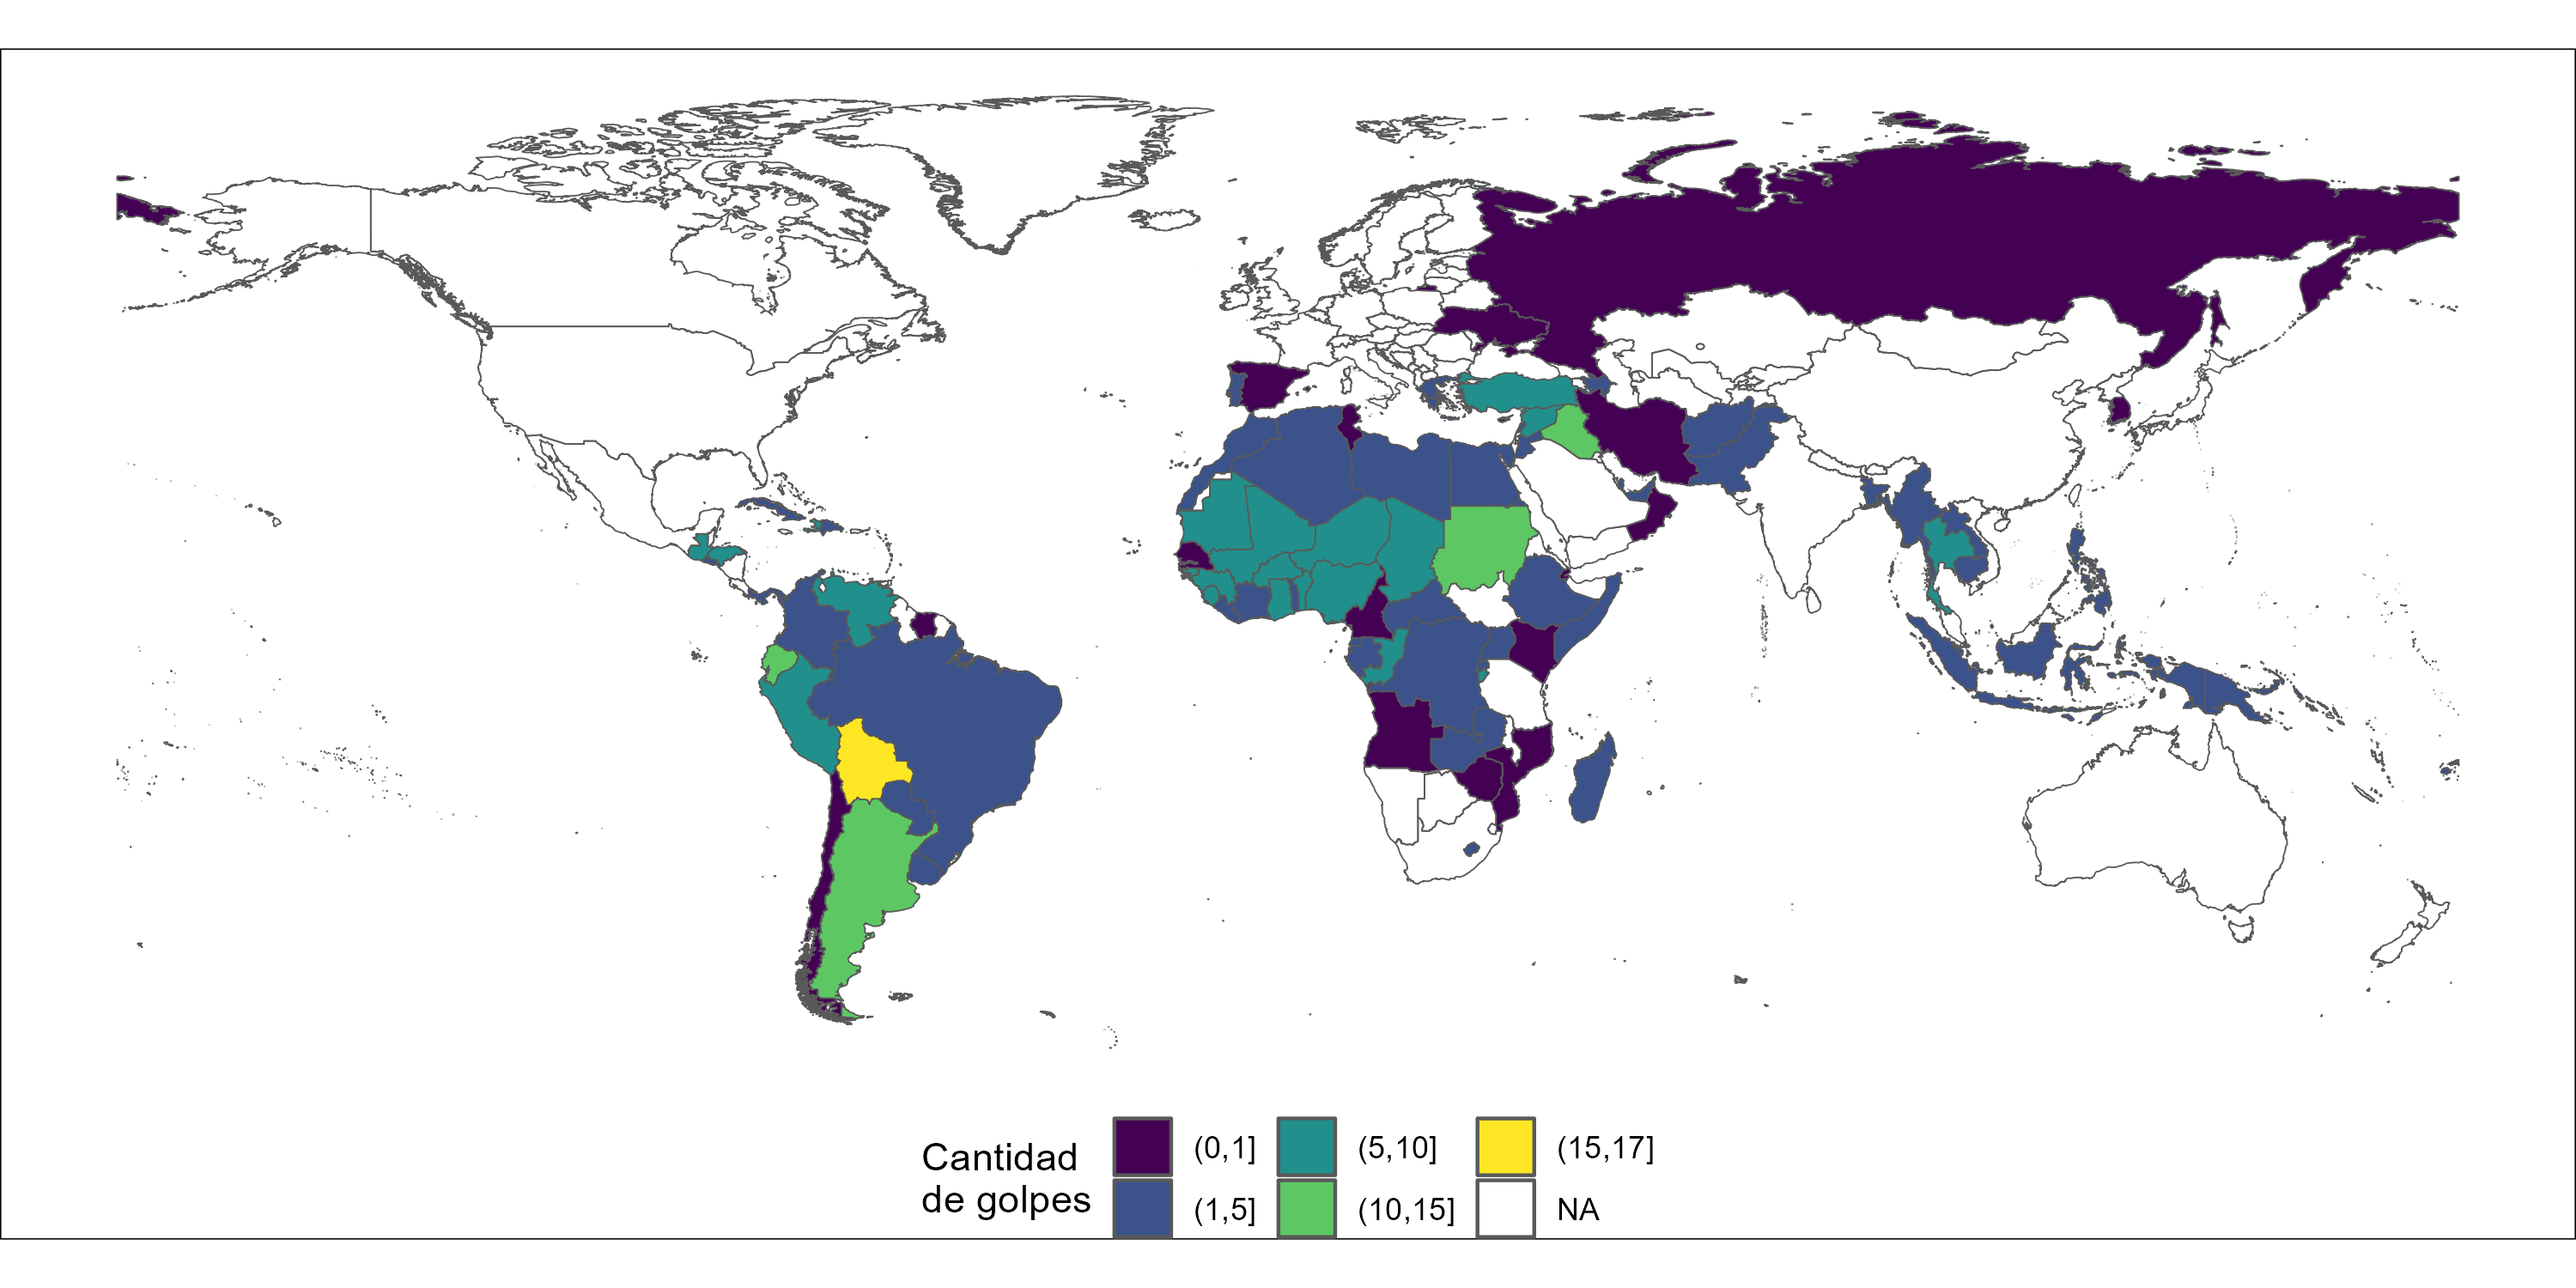
\includegraphics[width=1\textwidth]{2_golpes.png}
  \caption{Conteo de golpes de estado en el mundo\label{fig::mapa_golpes}}
\end{figure}

Con mayor precisión, observamos que la región del Sahel se destaca con respecto a sus
vecinos africanos. Los países en donde más golpes de estado se han producido son
Bolivia (17), Sudán (14), Argentina (13), Ecuador (11), Iraq (11), Siria(11), 
Guatemala (10) y Tailandia (10).

Desagregando por década se observan algunos cambios, así como la persistencia en 
algunas regiones. La región del Sahel y varias naciones circundantes fueron 
persistentemente afectadas por golpes de estado desde los años 60. En América del 
Sur, en cambio, la presencia casi total de situaciones golpistas en la región se 
fue acotando a partir de los años 80 hasta finalmente desaparecer en el siglo 
xxi. Para observar con más detalle y discriminado por años y países se puede ver 
la figura ~\ref{fig:golpes_anios}.

\begin{figure}[H]
  \centering  
  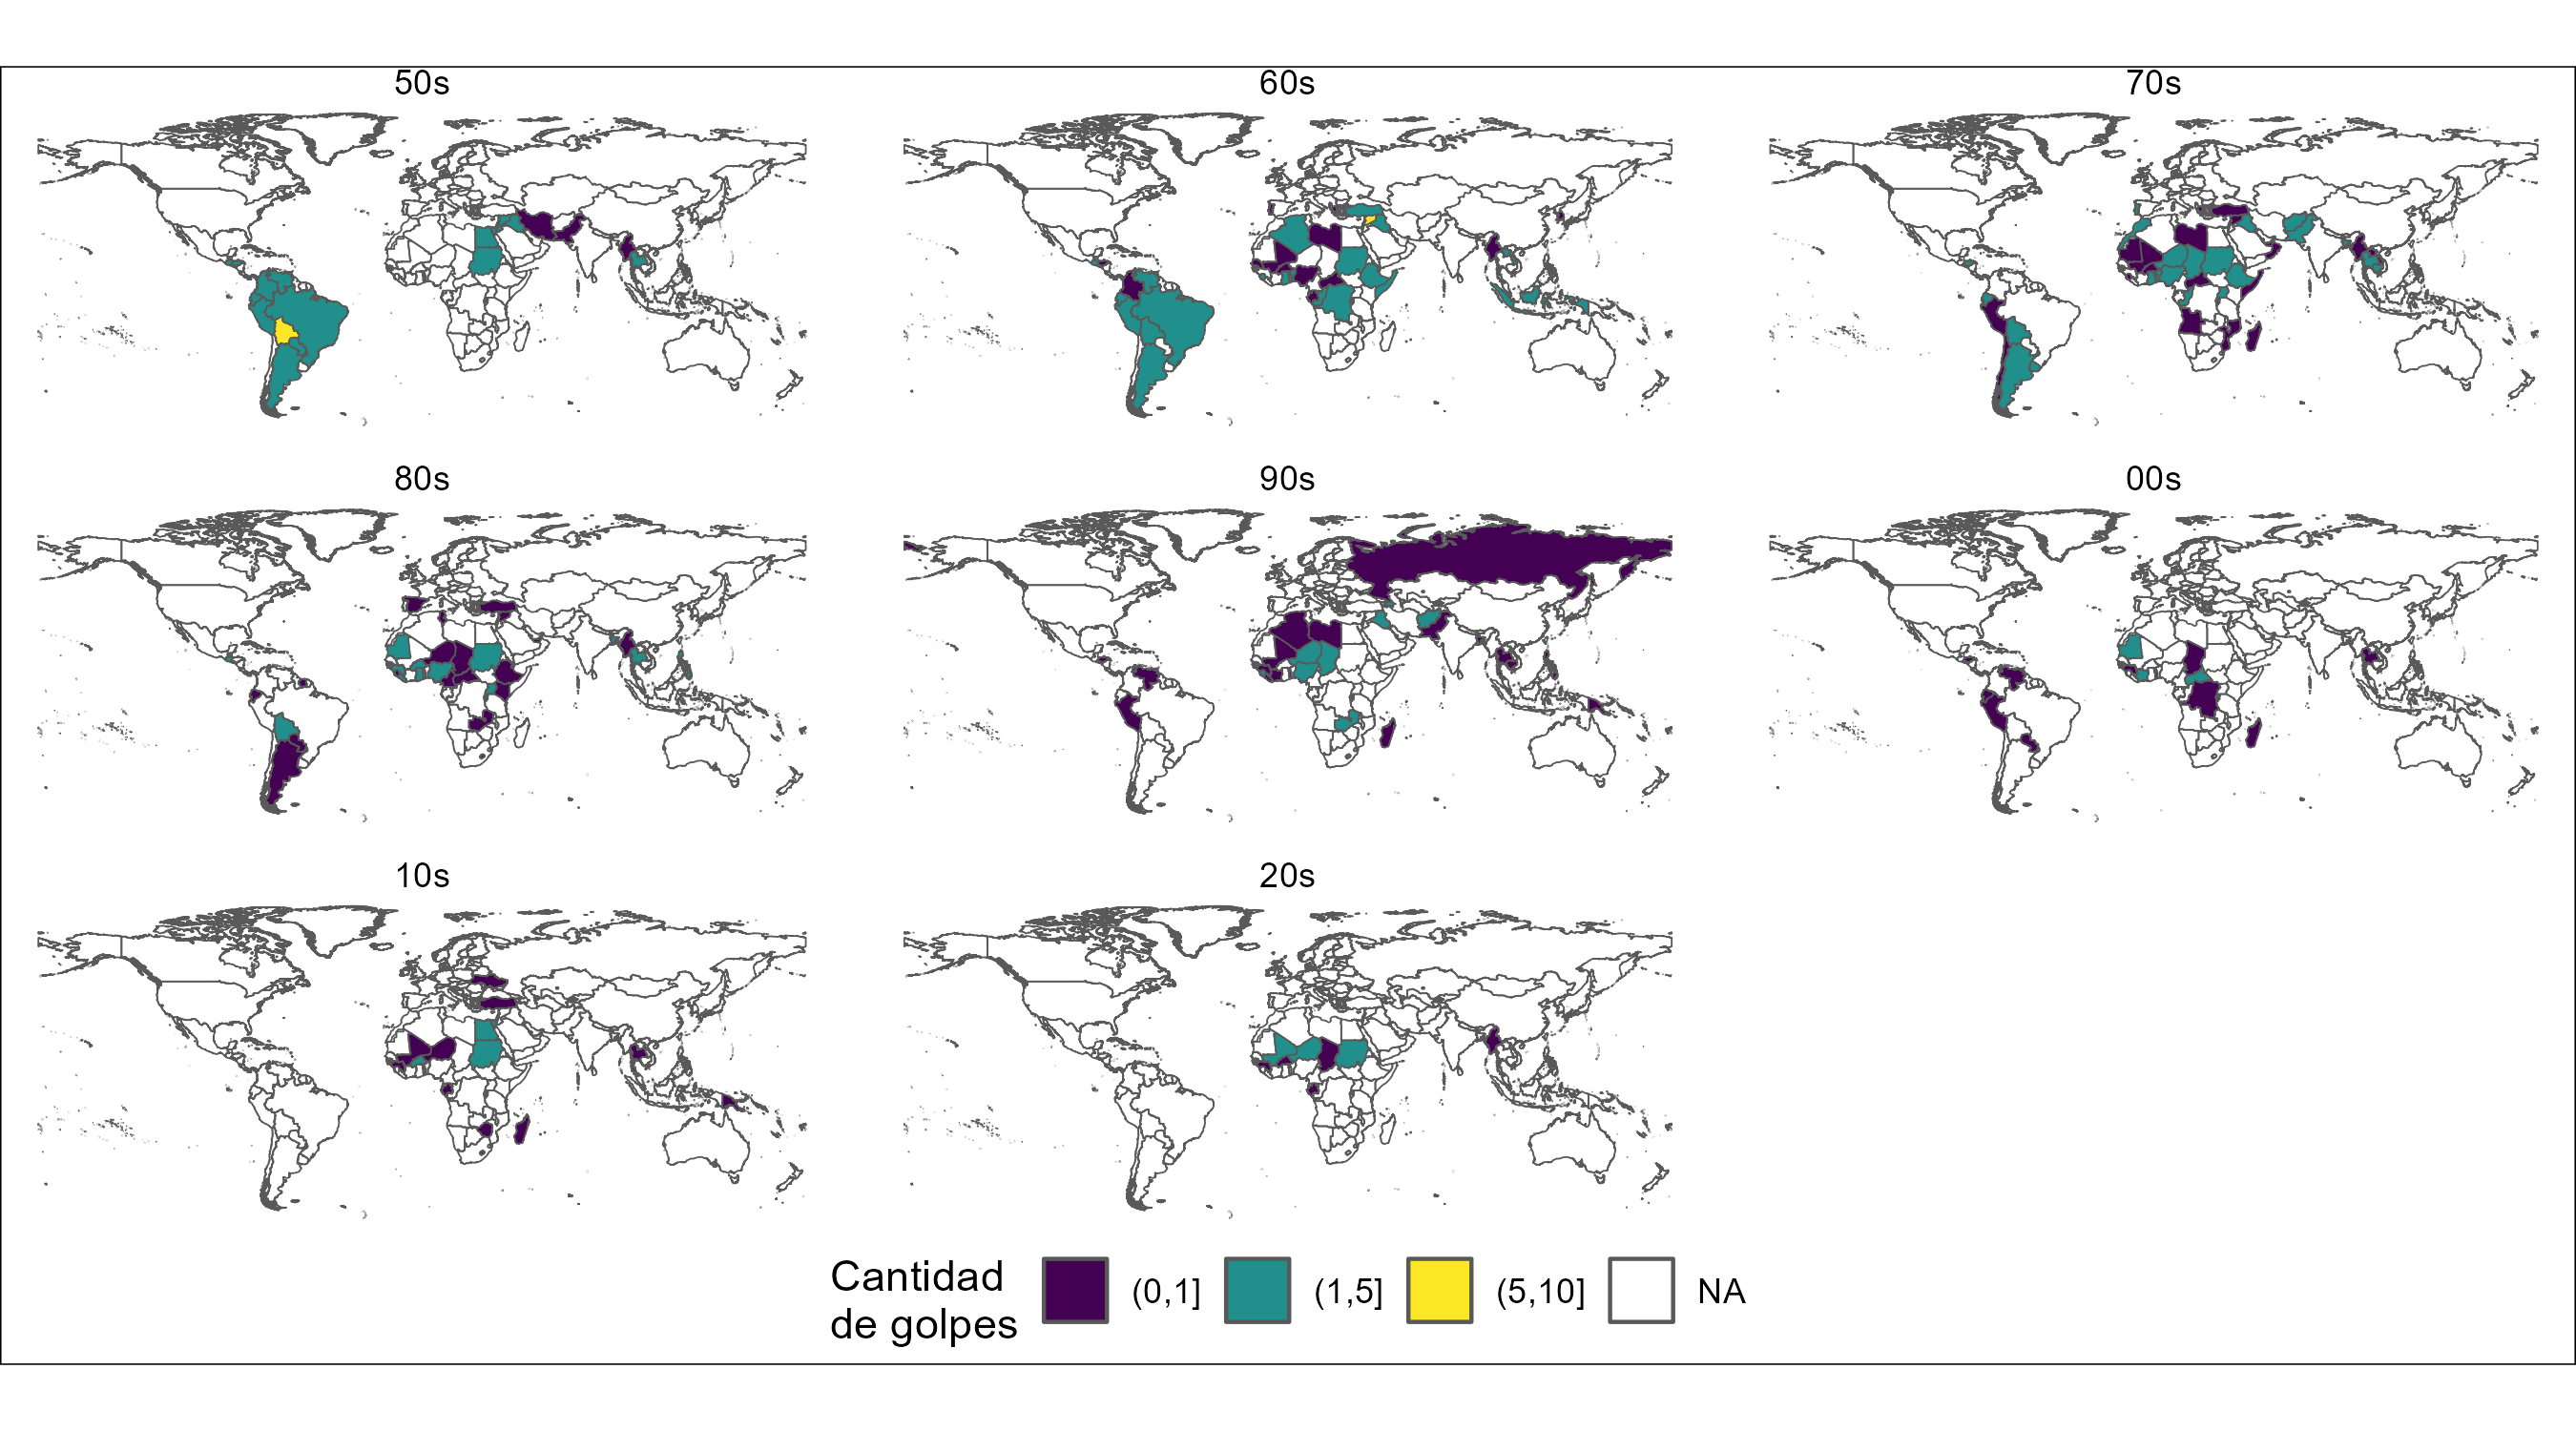
\includegraphics[width=1\textwidth]{3_golpes_decadas.png}
  \caption{Conteo de golpes por década}
\end{figure}

\section{Correlación entre variables}

Puesto que el dataset (previo filtrado de variables que no se utilizarán para
el entrenamiento) cuenta con alrededor de 1000 columnas, se vuelve imposible
realizar un mapa de calor que cruce todas las variables entre ellas (en la figura 
\ref{fig:correlacion_tot} dentro del anexo se muestra una tabla de correlacion de las 
variables individuales, agrupadas por el grupo de variable al que pertenecen). Por lo 
tanto, recurriremos al agrupamiento de variables provisto por el codebook para rezliar un
gráfico de correlación entre los promedios de grupos de variables, como se puede 
apreciar en la figura ~\ref{fig:correlacion_gp}.
\begin{figure}[H]
  \centering  
  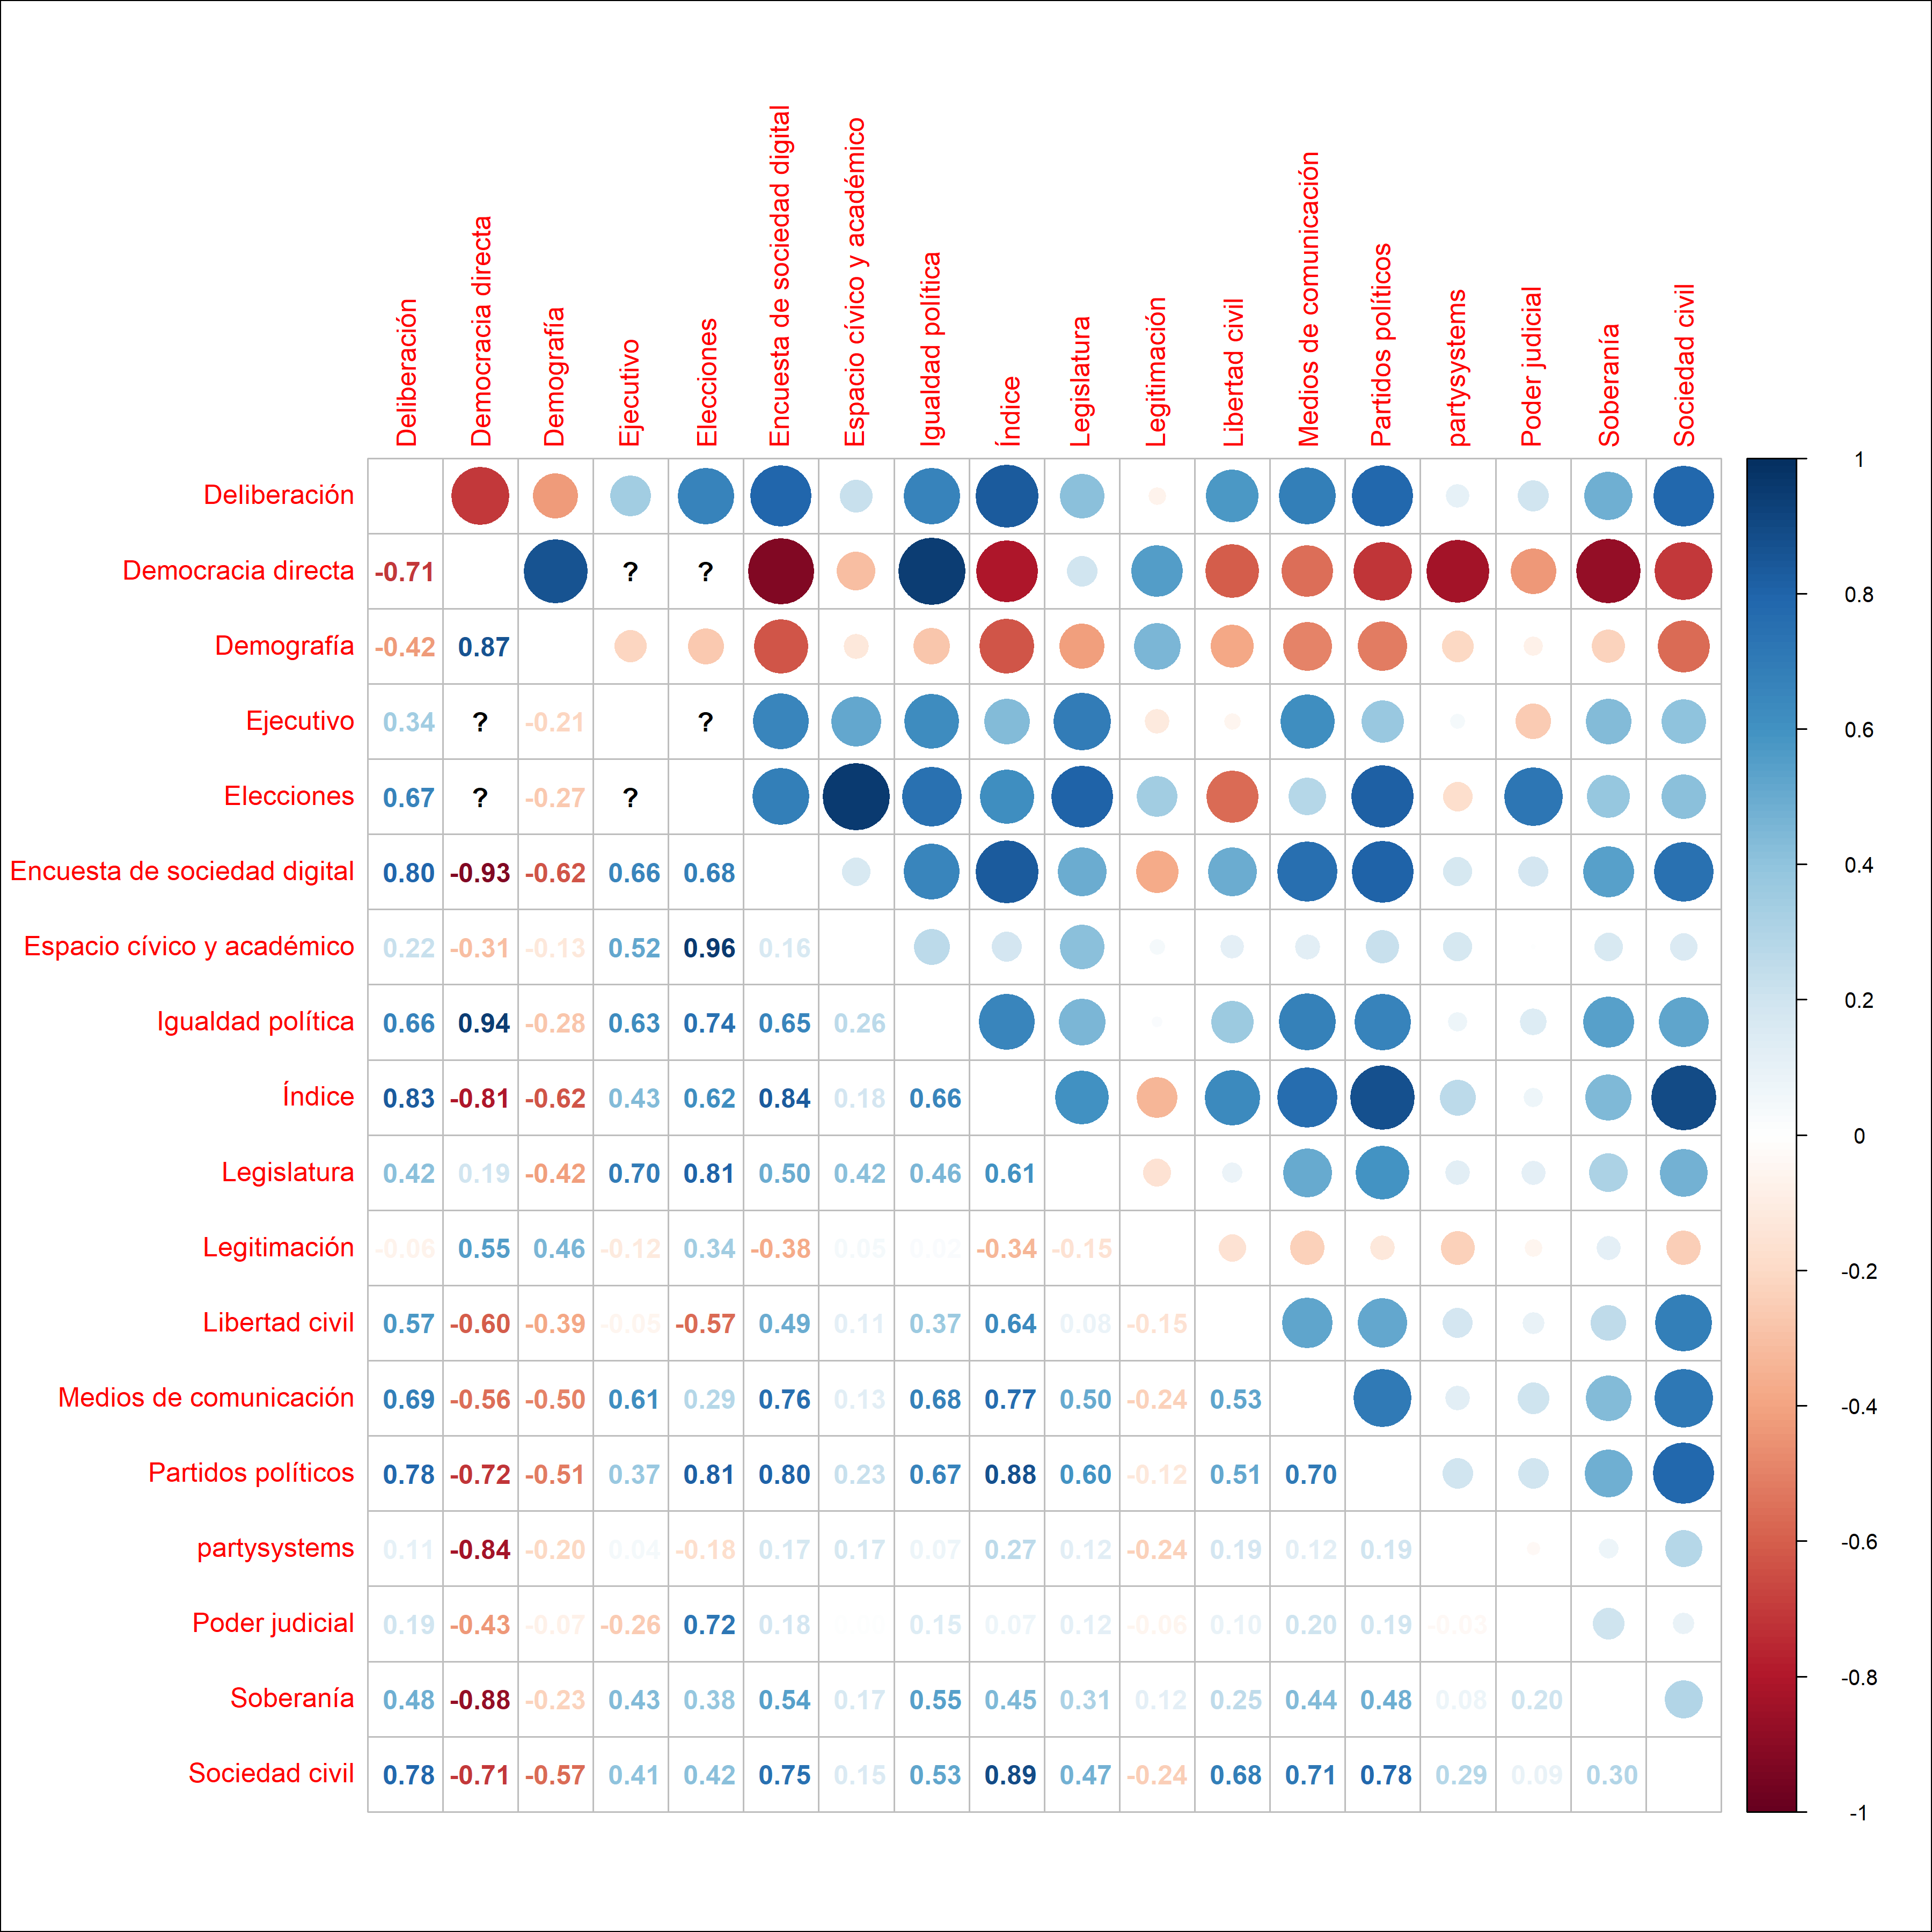
\includegraphics[width=1\textwidth]{5_correlacion_grupos.png}
  \caption{Correlación entre promedios de grupos de variables\label{fig:correlacion_gp}}
\end{figure}

%TODO intentar concluir algo de esto
De este gráfico podemos destacar la alta correlación negativa que el grupo
'democracia directa' tiene con varios grupos: 'encuesta de sociedad digital', con el 
grupo de los 'índices', el de 'partidos políticos', el de 'partysystems', el de 
'soberanía' y con el de 'sociedad civil'. Por otro lado, correlaciona fuertemente 
pero de manera positiva con los grupos de 'demografía' e 'igualdad política'. Por último, 
otras fuertes correlaciones a mencionar son entre el grupo 'elecciones' y 'espacio cívico 
y académico', entre el de 'sociedad civil' y el de 'índice', entre 'partidos políticos' e
'índice'. Tiene sentido que el grupo Índice correlacion con otros, puesto a que está
conformado por otras variables pertenecientes a los mismos.

\section{Anexo}

\begin{figure}[H]
  \centering  
  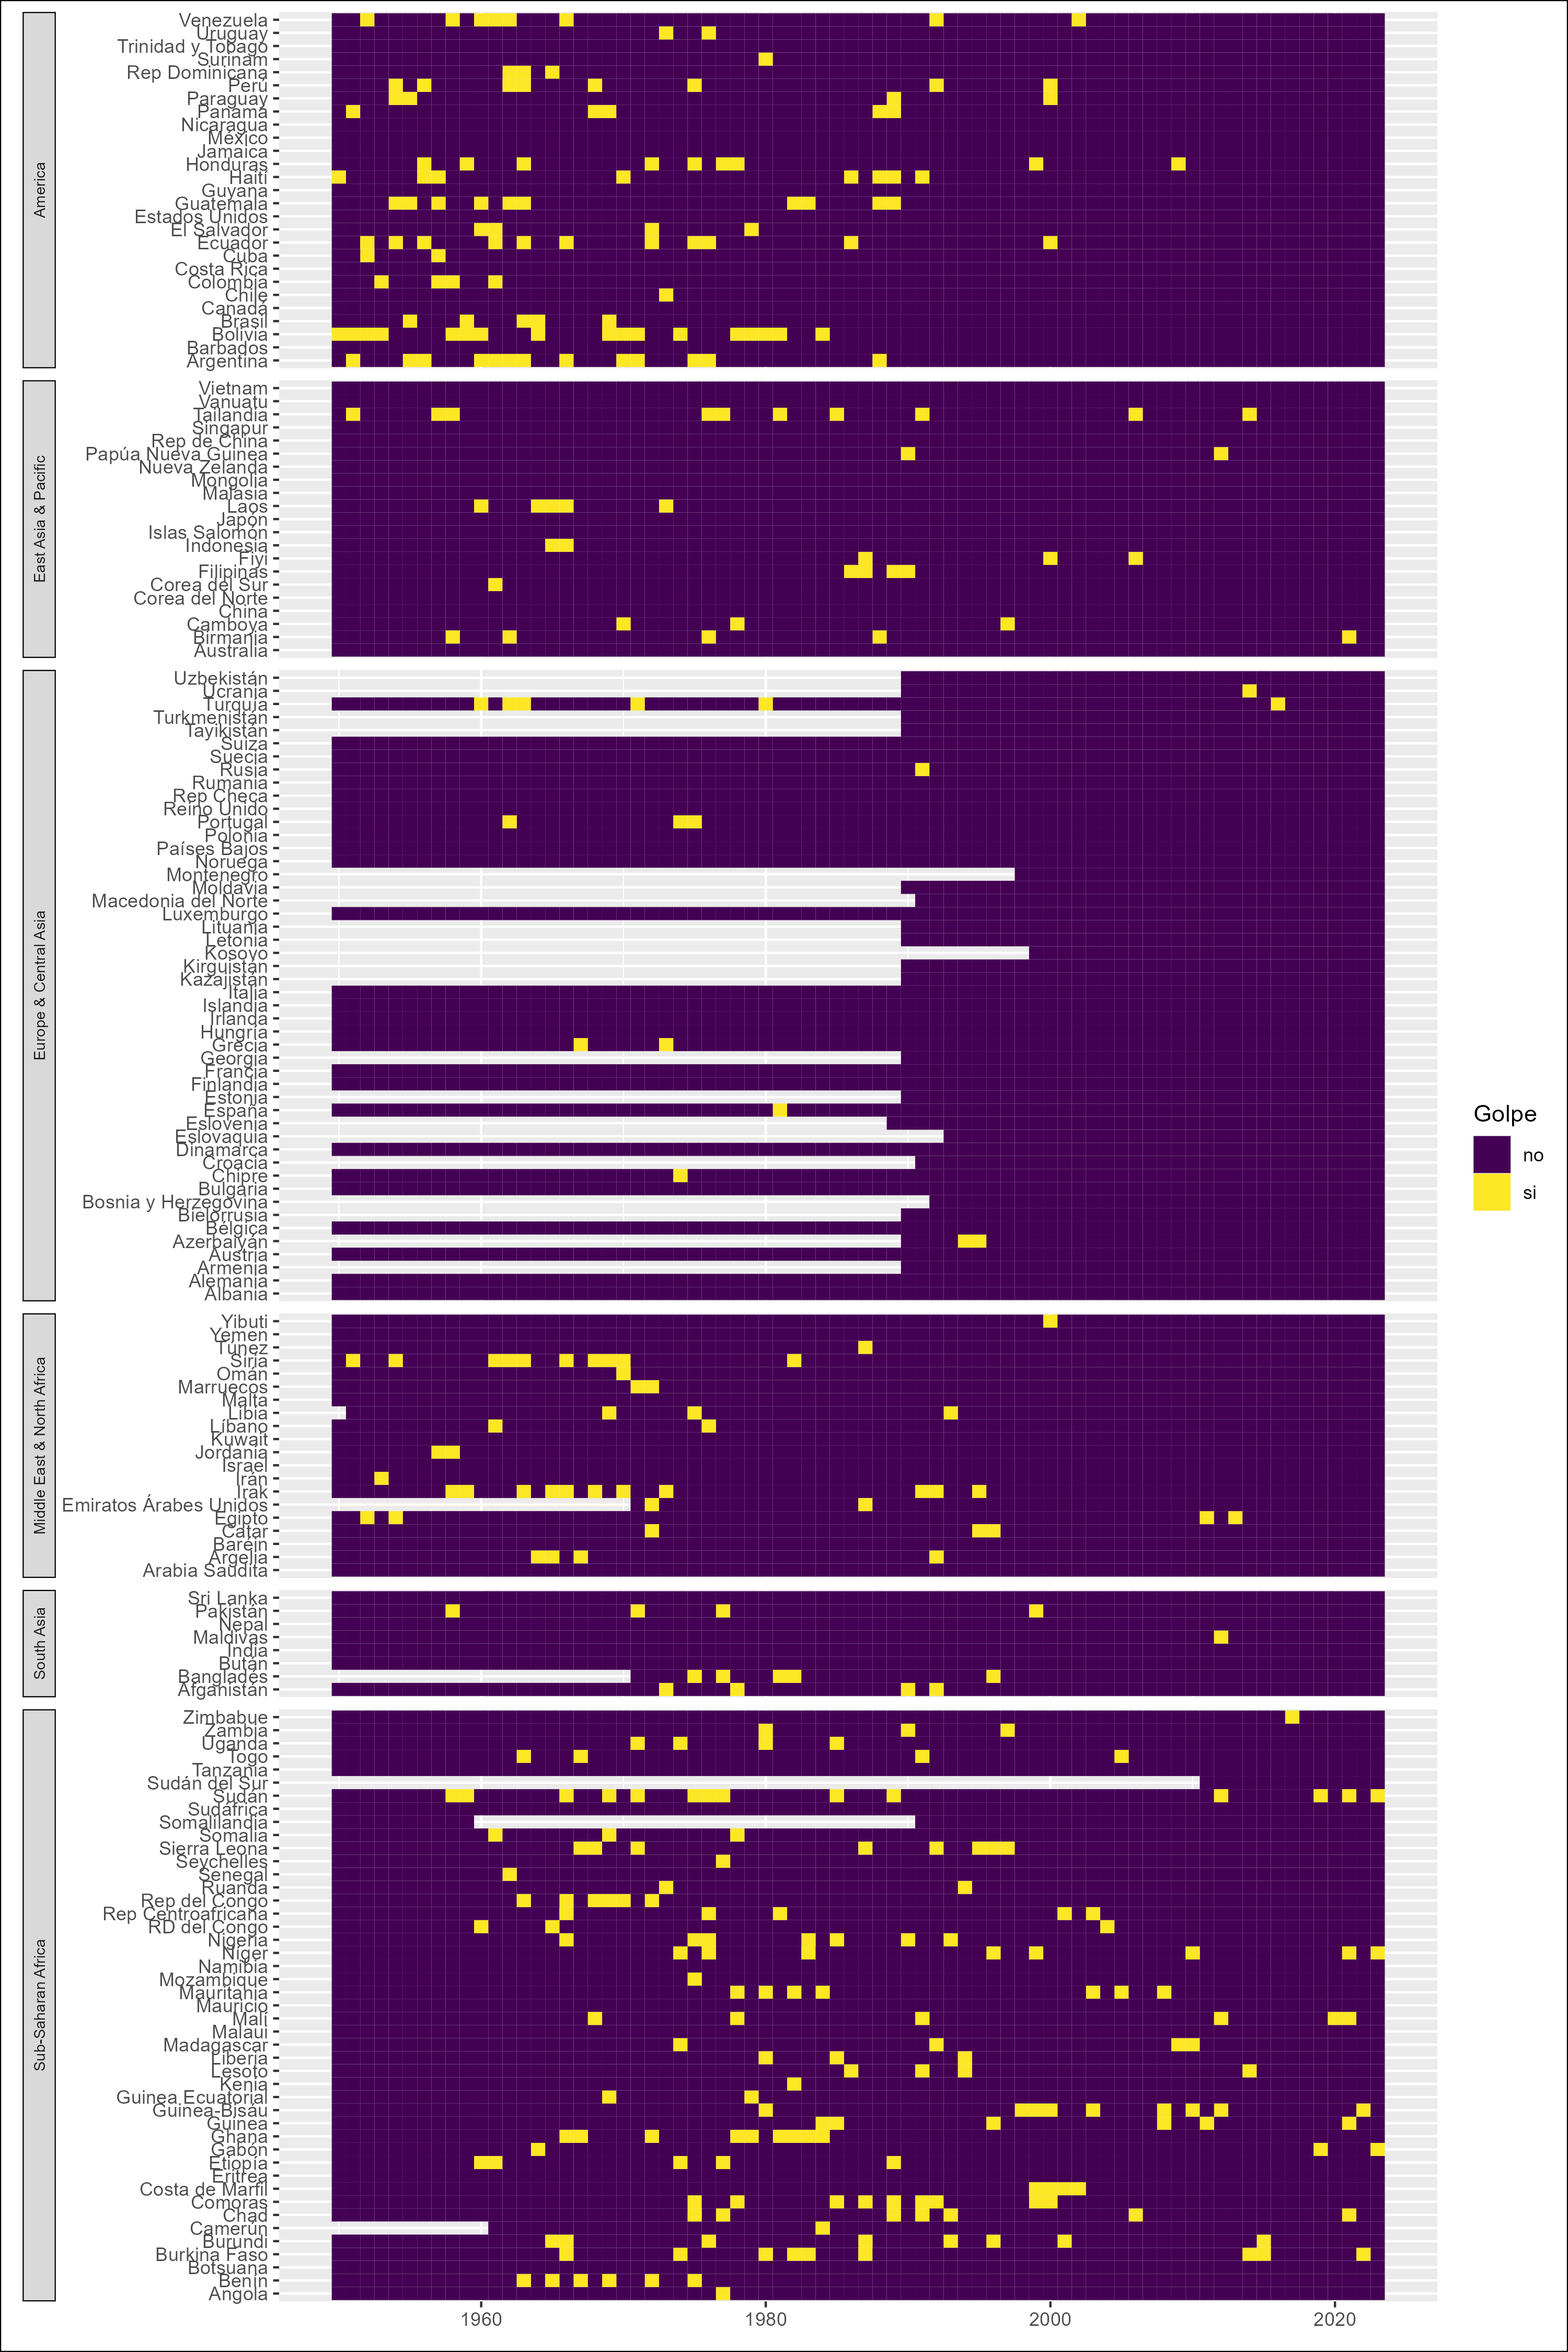
\includegraphics[width=1\textwidth]{4_golpes_anios.png}
  \caption{Conteo de golpes por año y región\label{fig:golpes_anios}}
\end{figure}

\begin{figure}[H]
  \centering  
  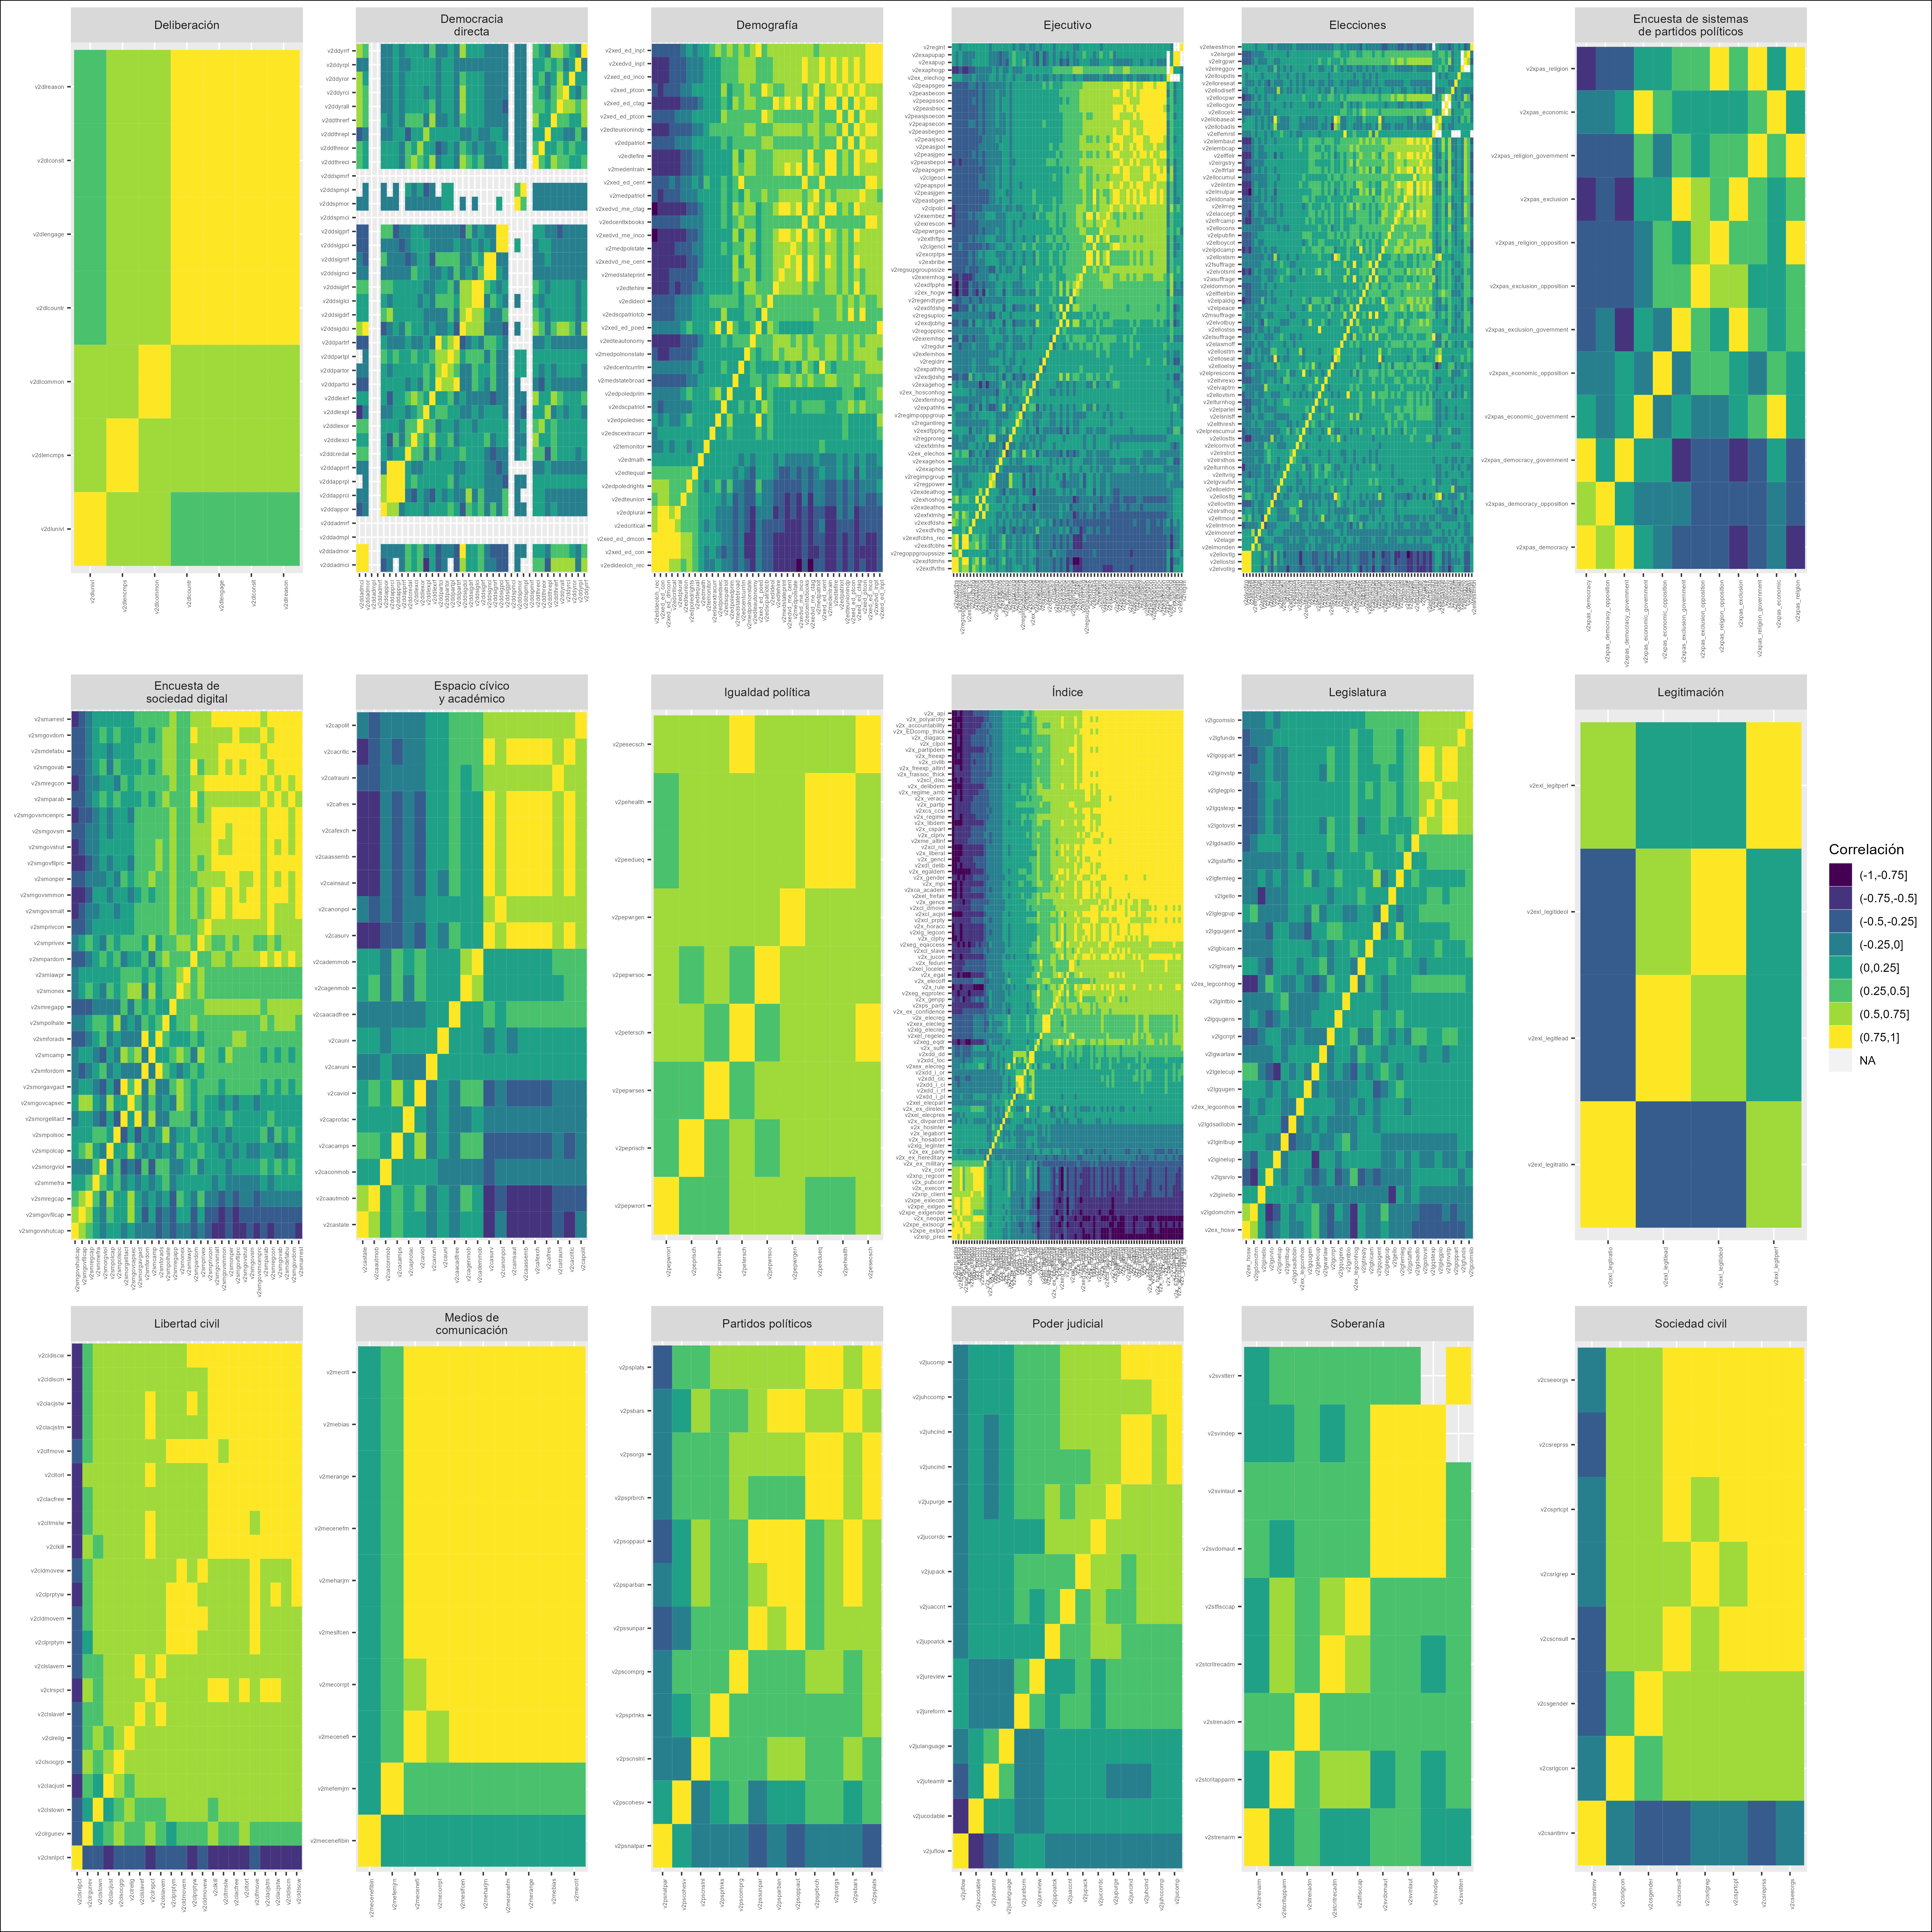
\includegraphics[width=1\textwidth]{6_correlacion.png}
  \caption{Correlación entre variables por grupo\label{fig:correlacion_tot}}
\end{figure}

\printbibliography

\end{document}